% !TEX root = Master.tex

We will start the pairwise analysis with inspecting the \ac{GJRM} approach. As mentioned above, the marginals are specified as Dagum distributed \acp{RV} and we choose the Student's t copula (the degrees of freedom do not affect the outcome, as they just serve as starting values for \ac{GAMLSS} estimation). All model parameters are set to constant, except the copula parameter (which is defined as in \autoref{eq:gjrm_kcc}). These settings also hold for Subsections \ref{sssec:kcc_28} and \ref{sssec:kcc_68}. We can see in the diagnostic plots of \autoref{fig:margin_estimates_kcc_26} that this type of model fitting returns quite successful results. \\

\begin{figure}[H]
\centering
  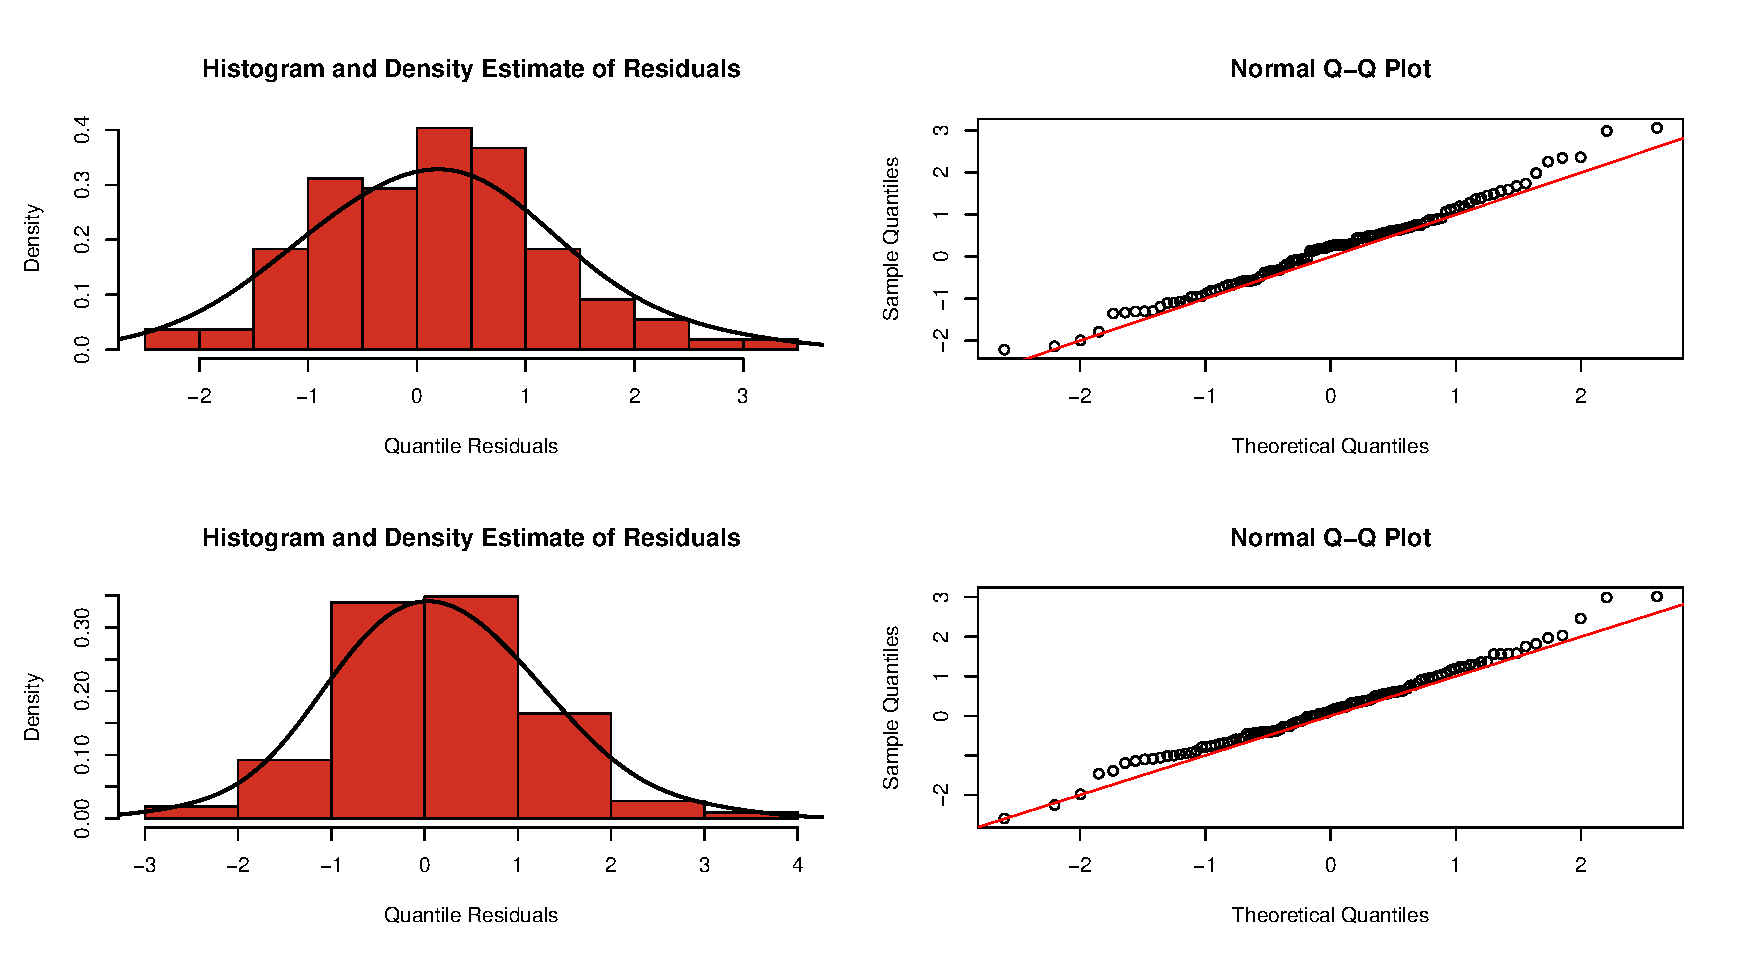
\includegraphics[width=0.9\linewidth]{figures/margin_estimates_kcc_26.eps}
  \caption{Estimation diagnostics for the response marginals KCC 2 \& KCC 6; \ac{GJRM} approach}
  \label{fig:margin_estimates_kcc_26}
\end{figure}

Regarding the fitting of the copula parameter $\rho$, time-varying estimation is achieved. The red line in \autoref{fig:copula_parameters_26} shows the estimated time-dependent sequence of $\hat{\rho}$, where an instant positive conclusion is that the outcome is very close to the gamCopula approach. This indicates that the model setup of these two approaches both agree for the most part on the dependence structure. (Confidence intervals of the lines are not shown to retain clarity in the figure).\\


\begin{figure}[H]
\centering
  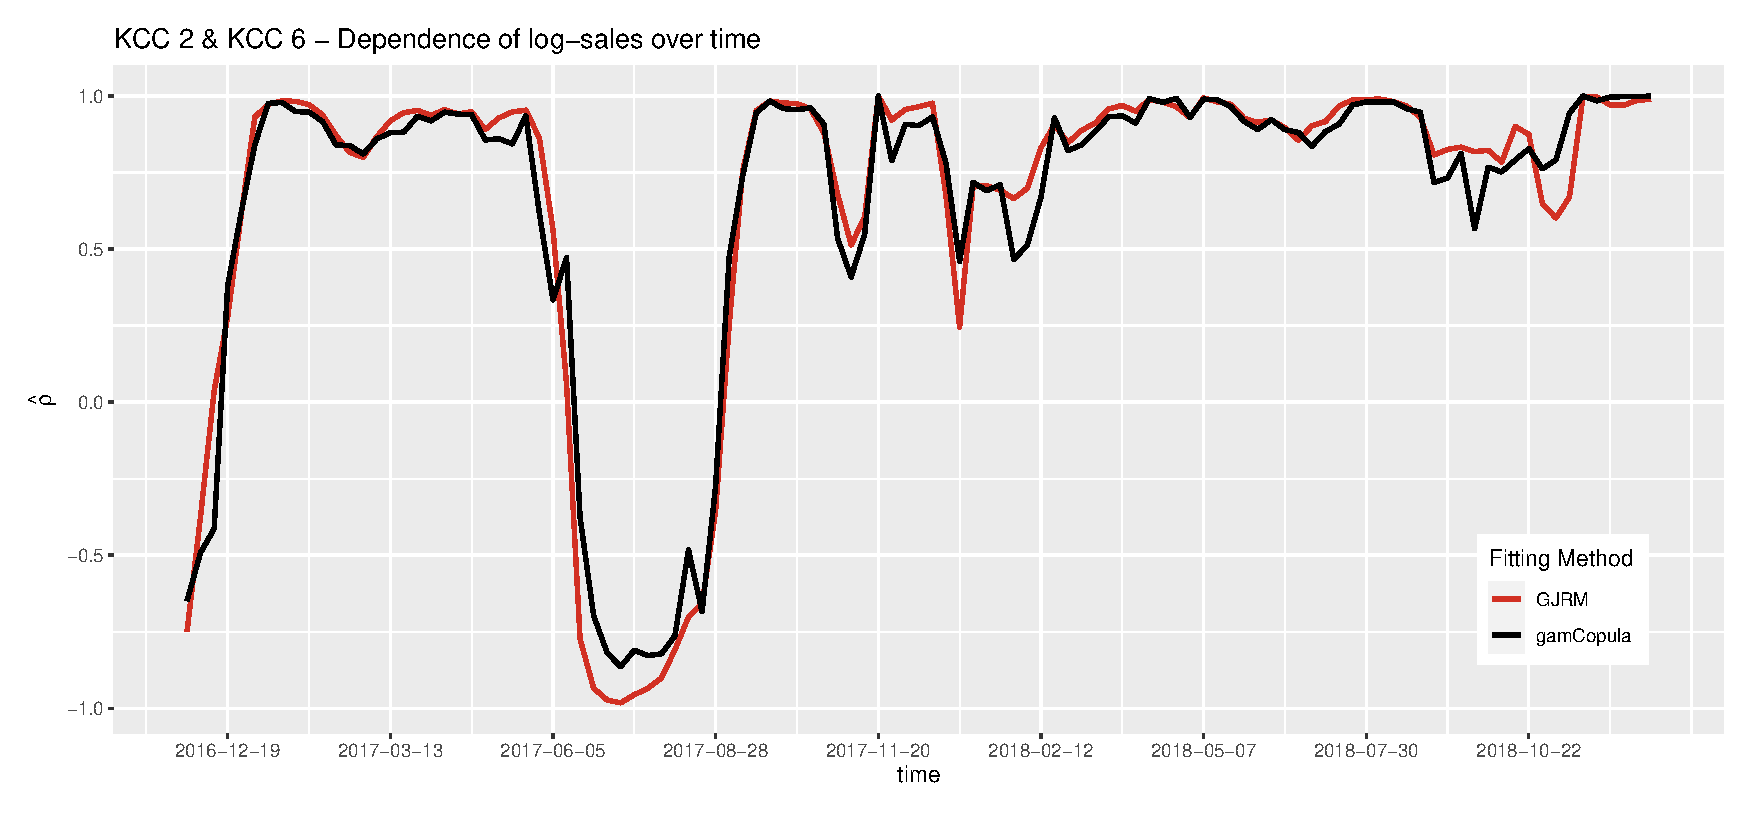
\includegraphics[width=0.9\linewidth]{figures/copula_parameters_26.eps}
  \caption{Estimated time-varying Pearson's correlation coefficients for the pair KCC 2 \& KCC 6}
  \label{fig:copula_parameters_26}
\end{figure}


By large, the dependence is constantly at a very high positive level, with a noticeable turn in high negativity during the summer months of 2017. The gamCopula approach seems to pick up slightly more regional fluctuations than the \ac{GJRM} approach.






